% =================================================================================================
% File:			gestione_contenuti.tex
% Description:	Definisce la sezione relativa ad un capitolo del documento
% Created:		2015-04-25
% Author:		Santacatterina Luca
% Email:		santacatterina.luca@mashup-unipd.it
% =================================================================================================
% Modification History:
% Version		Modifier Date		Change											Author
% 0.0.1 		2015-05-245			inizio stesura sezione capitolo					Santacatterina Luca
% =================================================================================================
%

% CONTENUTO DEL CAPITOLO

\section{Gestione contenuti} % (fold)
\label{sec:gestione_contenuti}
	Dopo aver eseguito le istruzioni per l'autenticazione viene visualizzata la dashboard dell’applicazione.\newline
	Nella schermata principale della dashboard vengono visualizzati in riquadri le \textbf{recipes} disponibili nel sistema (Figura: \ref{fig:ricette_disponibili}), mentre nella sinistra dell'applicazione è disponibile il menù principale di gestione (Figura: \ref{fig:menu_principale_utente})
	\begin{figure}[H]
		\centering
		\centerline{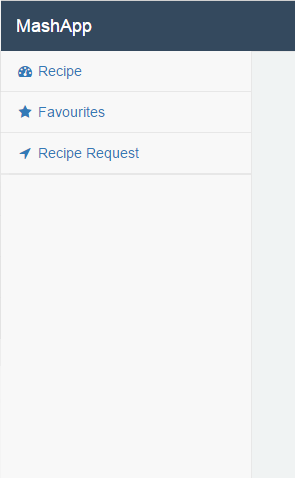
\includegraphics[width=6cm]{images/menu_principale_utente.png}}
		\caption{Dashboard - Menù principale}
		\label{fig:menu_principale_utente}
	\end{figure}



	\pagebreak
	\subsection{Gestione ricette} % (fold)
	\label{sec:gestione_ricette}
		Nel pannello principale si visualizzano tutte le recipes (Figura: \ref{fig:ricette_disponibili}) presenti nell'applicazione.\newline
		Per ogni recipe vengono fornite due operazioni:
		\begin{itemize}
			\item \textbf{Show metrics}: permette la visualizzazione di tutte le metrics di una determinata recipe;
			\item \textbf{Compare metrics}: permette la comparazione di più recipes aventi in comune la stessa categoria.
		\end{itemize}

		\begin{figure}[H]
			\centering
			\centerline{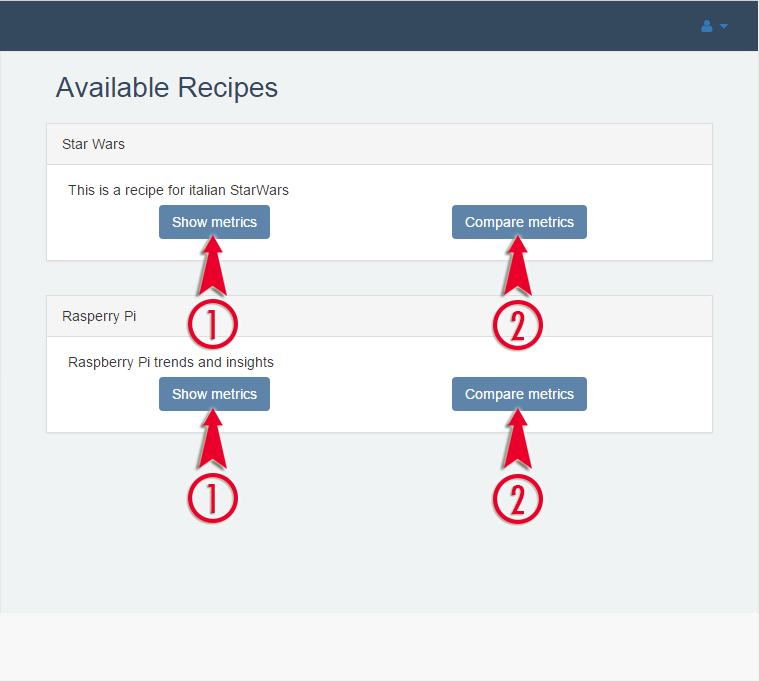
\includegraphics[width=14cm]{images/ricette_disponibili.png}}
			\caption{Dashboard - Ricette disponibili}
			\label{fig:ricette_disponibili}
		\end{figure}


		\pagebreak
		\subsubsection{Visualizzazione metriche} % (fold)
		\label{sec:visualizzazione_metriche}
			Nella schermata (Figura: \ref{fig:visualizzazione_metriche}) vengono elencate tutte le metriche disponibili dei vari social network presi in analisi.\newline
			Per ogni social network è riservata una scheda di navigazione. Selezionando i tab si visualizzano le metriche associate.\newline
			Ogni metrica nell'elenco visualizza titolo, tipo e pulsante per la generazione dei grafici.
			\begin{figure}[H]
				\centering
				\centerline{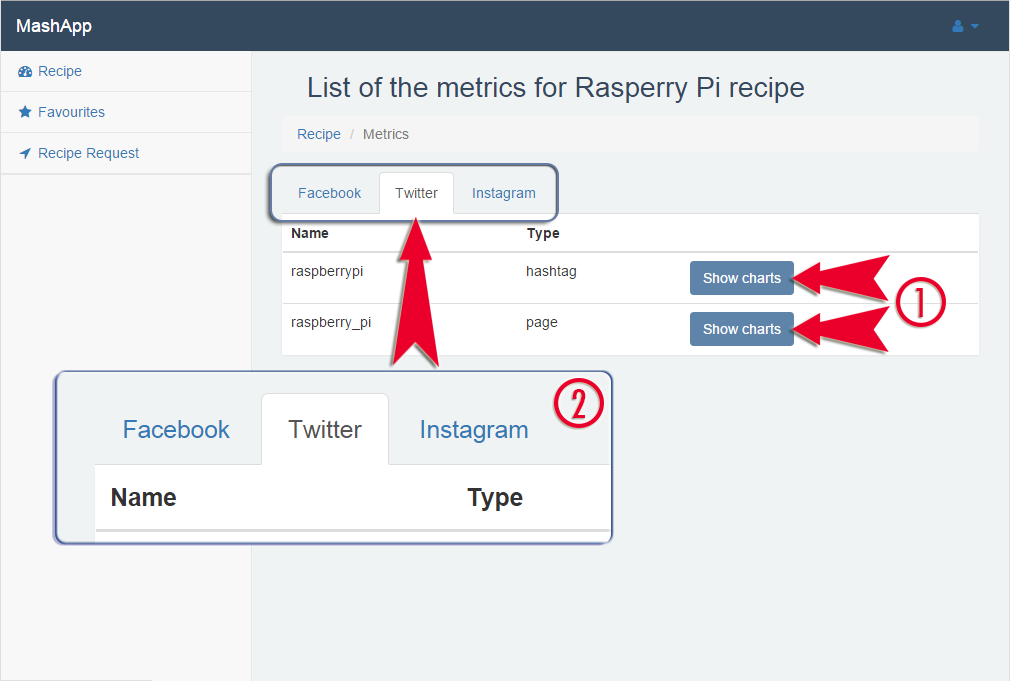
\includegraphics[width=14cm]{images/visualizzazione_metriche.png}}
				\caption{Visualizzazione metriche disponibili}
				\label{fig:visualizzazione_metriche}
			\end{figure}
		% section Visualizzazione metriche (end)


		\subsubsection{Visualizzazione grafici metriche} % (fold)
		\label{sec:visualizzazione_grafici_metriche}
			Premendo il pulsante di generazione dei grafici (Figura: \ref{fig:visualizzazione_metriche}) si accede ad una nuova pagina dedicata alla visualizzazione dei dati (Figura: \ref{fig:visualizzazione_grafici_metriche}).
			\begin{figure}[H]
				\centering
				\centerline{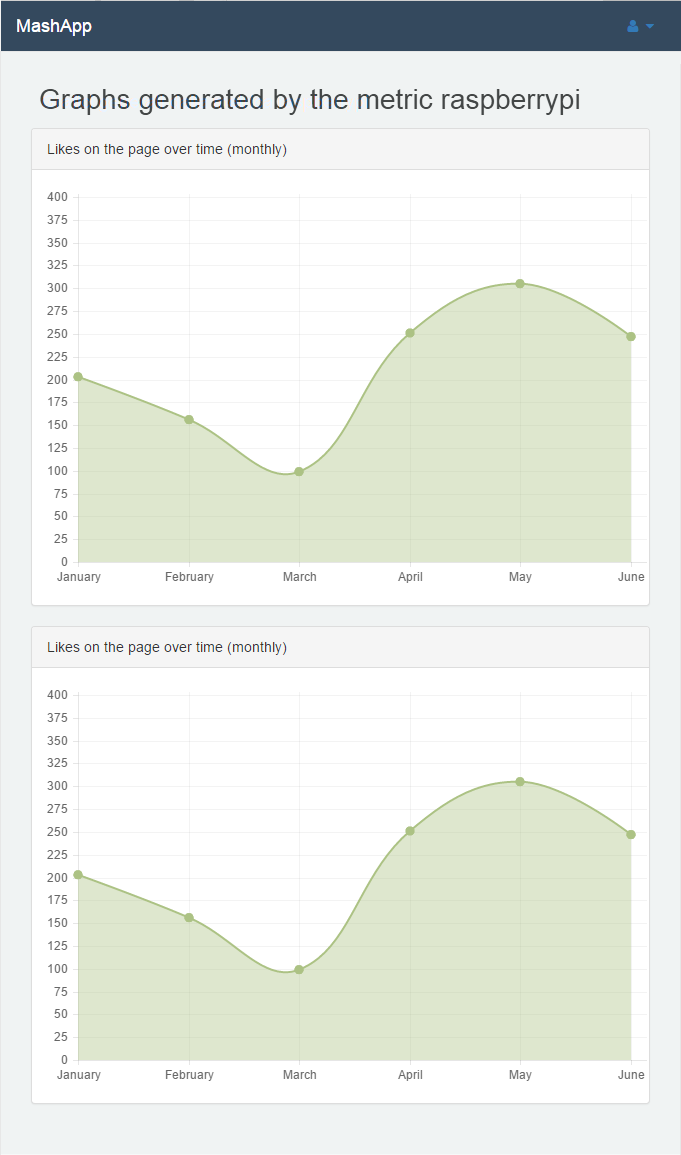
\includegraphics[width=14cm]{images/visualizzazione_grafici_metriche.png}}
				\caption{Visualizzazione grafici metriche disponibili}
				\label{fig:visualizzazione_grafici_metriche}
			\end{figure}
			Per ogni metrica sono disponibili vari grafici. Questi possono variare in base alla tipologia di metrica applicata.\newline
			Le tipologie di grafico possibili possono essere:
			\begin{itemize}
				\item Line Chart;
				\item Bar Chart;
				\item Doughnut Chart;
				\item Radar Chart;
				\item Pie Chart;
				\item Polar Area Chart;
				\item Dynamic Chart;
				\item Map Chart.
			\end{itemize}
		% section Visualizzazione grafici metriche (end)


		\pagebreak
		\subsubsection{Comparazione metriche} % (fold)
		\label{sec:comparazione_metriche}
			Premendo il pulsante di comparazione delle metriche (Figura: \ref{fig:visualizzazione_metriche}) si accede ad una nuova pagina contenente la sezione dedicata alla configurazione delle metriche da confrontare (Figura: \ref{fig:comparazione_metriche}).
			\begin{figure}[H]
				\centering
				\centerline{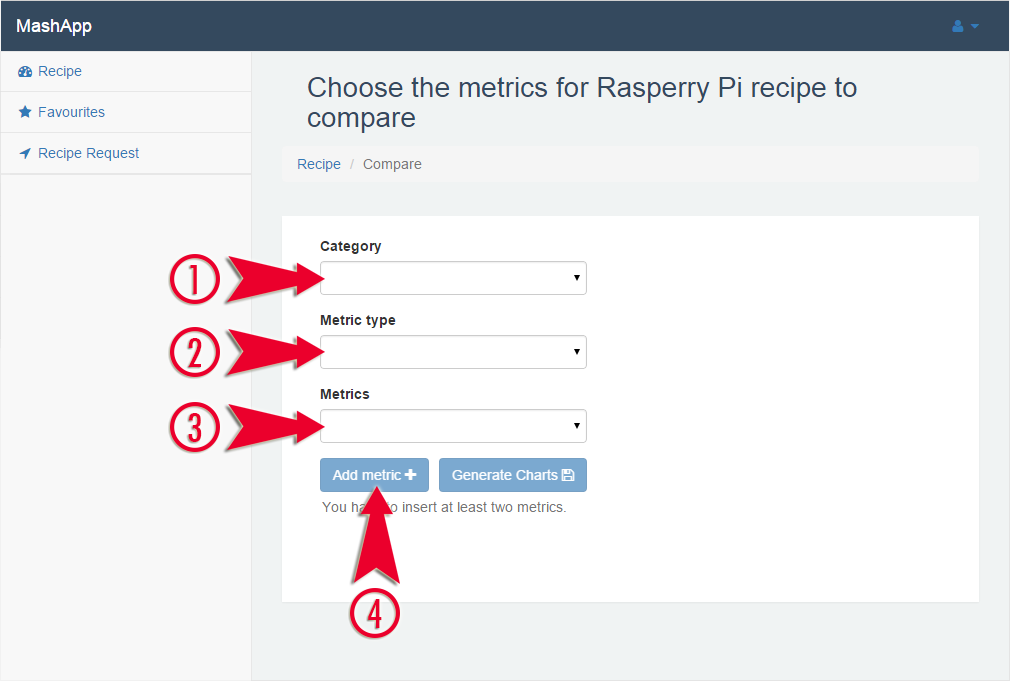
\includegraphics[width=14cm]{images/comparazione_metriche.png}}
				\caption{Comparazione metriche}
				\label{fig:comparazione_metriche}
			\end{figure}
			All'interno della pagina si trovano tre campi form da completare scegliendo la tipologia di dati da comparare. Dopo la selezione, il pulsante \textbf{Add metric+} cambia di colore e si abilita, questo permette di aggiungere più metriche all'elenco di comparazione presente dopo la pressione del pulsante.\newline
			Possono essere aggiunte più metriche in base all'esigenza utente e in base a quelle disponibile nell'applicazione. Nella figura \ref{fig:esempio_comparazione_metriche} è possibile vedere un breve esempio di funzionamento.
			\begin{figure}[H]
				\centering
				\centerline{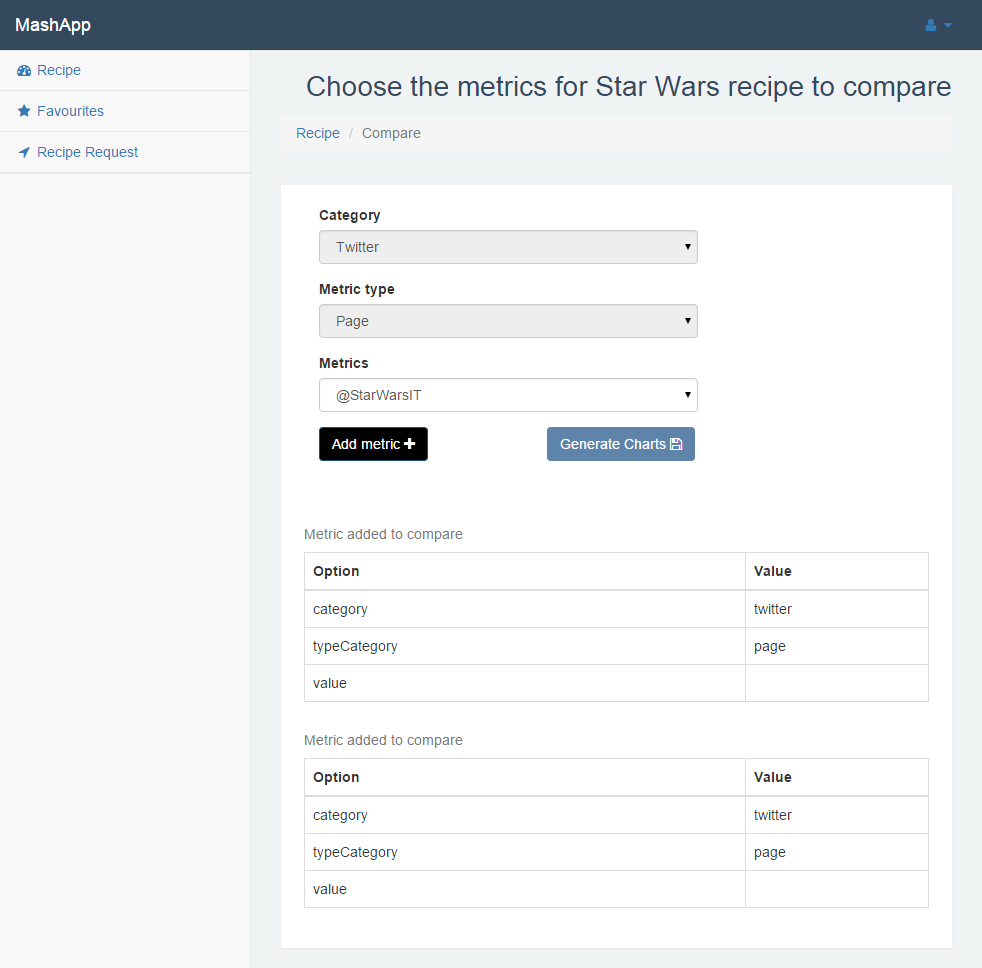
\includegraphics[width=14cm]{images/esempio_comparazione_metriche.png}}
				\caption{Esempio comparazione metriche}
				\label{fig:esempio_comparazione_metriche}
			\end{figure}
		% section Comparazione metriche (end)


		\subsubsection{Comparazione grafici metriche} % (fold)
		\label{sec:comparazione_grafici_metriche}
			Dopo aver eseguito i passi del capitolo precedente, il pulsante \textbf{Generate Charts} si sblocca. Premendolo, si carica una nuova pagina contenente i grafici di comparazione.\newline
			Sono disponibili solamente i grafici associati alle metriche che permettono tale funzionalità.
		% section Comparazione grafici metriche (end)

	% section Gestione ricette (end)


	\pagebreak
	\subsection{Gestione preferiti} % (fold)
	\label{sec:gestione_preferiti}
		Nella sezione \textbf{Favourites}, accessibile tramite il menu principale (Figura: \ref{fig:menu_principale_utente}) è possibile ottenere un elenco dei grafici nella quale è stata specificata la sezione di preferenza. Vengono raggruppati i grafici preferiti per una più veloce visualizzazione da parte dell'utente.\newline
		Per aggiungere i grafici alla sezione \textbf{Favourites} è necessaria la selezione nella relativa categoria.\newline
		Nella figura seguente è possibile visualizzare il grafico preferito di confronto tra due recipes:
		\begin{figure}[H]
			\centering
			\centerline{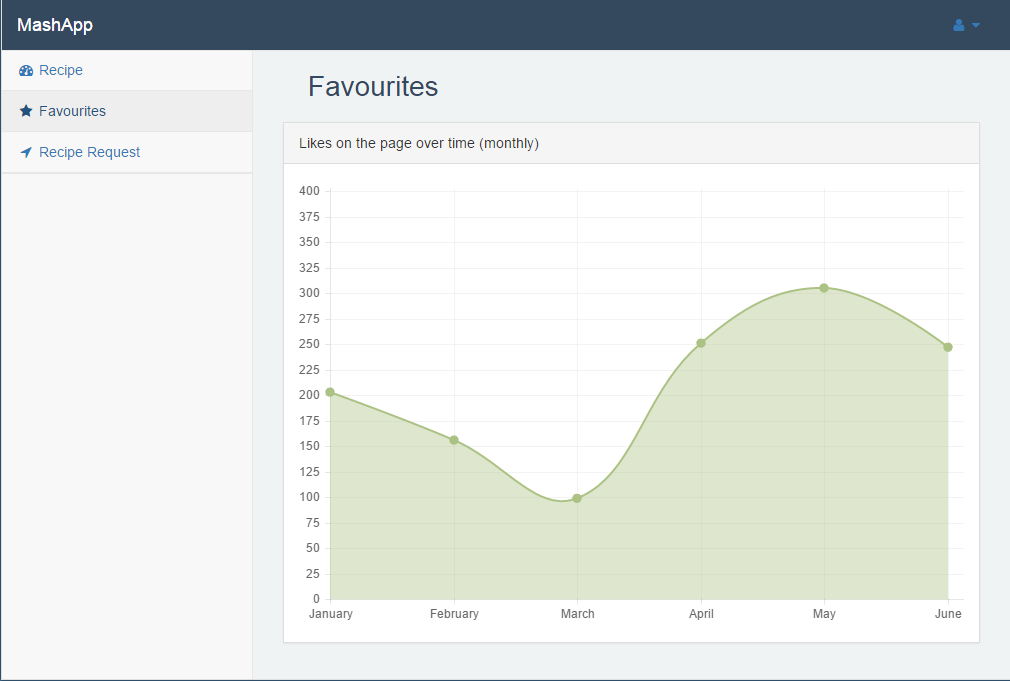
\includegraphics[width=14cm]{images/esempio_preferiti.png}}
			\caption{Esempio preferiti}
			\label{fig:esempio_preferiti}
		\end{figure}
	% section Gestione preferiti (end)


	\pagebreak
	\subsection{Richiesta nuove ricette} % (fold)
	\label{sec:Richiesta nuove ricette}
		Per richiedere una nuova recipe l'utente deve aprire una segnalazione agli amministratori di sistema.\newline
		Per poter accedere alla sezione \textbf{Request a new recipe} si deve cliccare sul menù principale (Figura: \ref{fig:menu_principale_utente}) alla voce \textbf{Recipe Request}.
		Si otterrà così il caricamento della nuova pagina (Figura: \ref{fig:richiesta_nuova_ricetta}). All'interno è presente un form da completare con i seguenti dati:
		\begin{itemize}
			\item \textbf{Recipe title}: inserire titolo recipe;
			\item \textbf{Recipe description}: inserire descrizione recipe ;
			\item \textbf{Category}: selezionare la categoria appartenente tra quelle disponibili;
			\item \textbf{Metric type}: selezionare la metrica associata alla categoria scelta precedentemente;
			\item \textbf{Value}: inserire il valore della metrica presente sul social network.
		\end{itemize}
		\begin{figure}[H]
			\centering
			\centerline{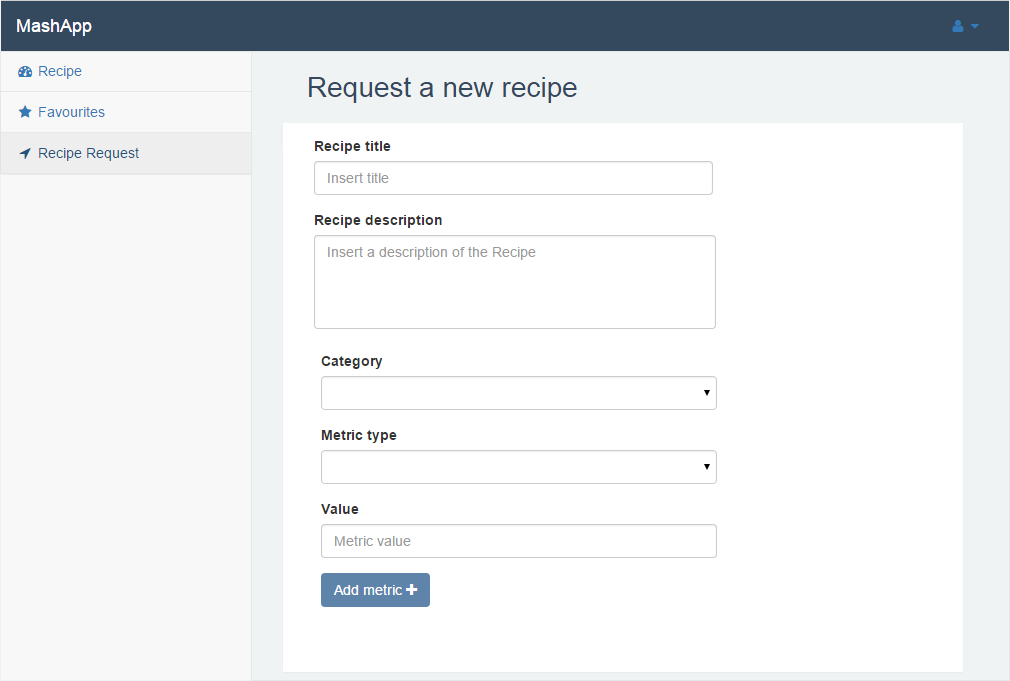
\includegraphics[width=14cm]{images/richiesta_nuova_ricetta.png}}
			\caption{Richiesta nuova ricetta}
			\label{fig:richiesta_nuova_ricetta}
		\end{figure}
	% section Richiesta nuove ricette (end)


% section Gestione contenuti (end)